\newcommand{\figMain}{
    %\begin{figure*}[t]
    %    \subfloat[\label{fig:main}]{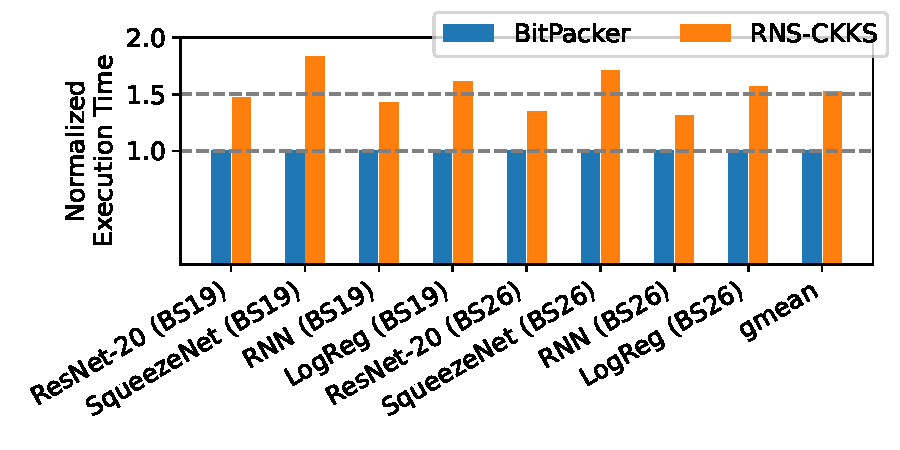
\includegraphics[width=\columnwidth]{plots/perf_main.pdf}}
    %    \hfill\subfloat[\label{fig:breakdown}]{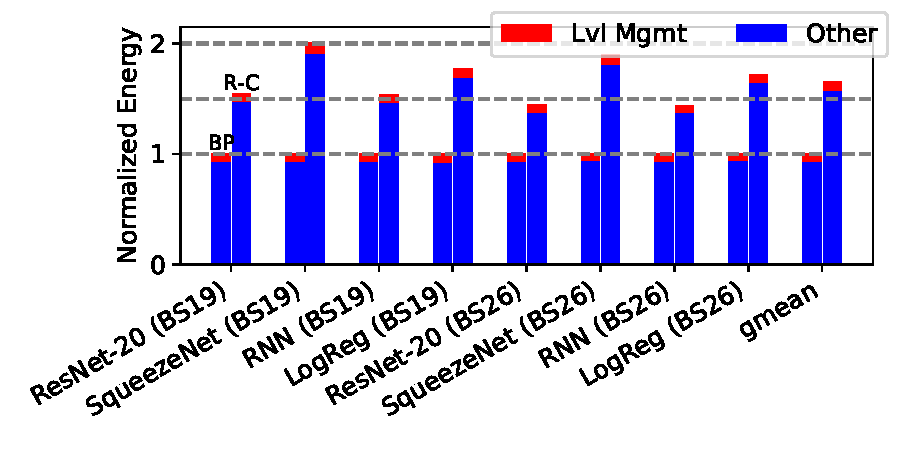
\includegraphics[width=\columnwidth]{plots/breakdown.pdf}}
    %    \caption{28-bit \name's (BP) performance (a) and energy (b) compared to 28-bit RNS-CKKS (R-C).}
    %\end{figure*}
    \begin{figure}[t]
      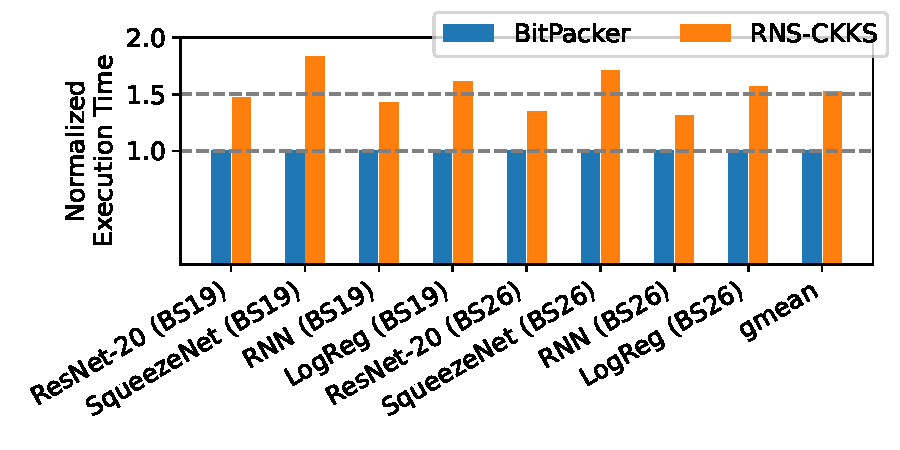
\includegraphics[width=\columnwidth]{plots/perf_main.pdf}
      \vspace{-0.35in}
      \caption{Execution time for \name and RNS-CKKS on CraterLake with 28-bit words (lower is better).}
      \label{fig:main}
      \vspace{-0.15in}
    \end{figure}
    \begin{figure}[t]
      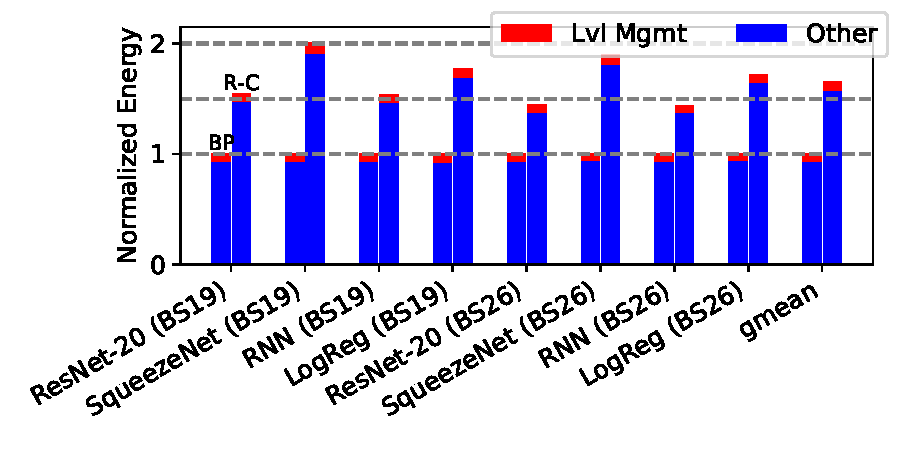
\includegraphics[width=\columnwidth]{plots/breakdown.pdf}
      \vspace{-0.35in}
      \caption{Energy for \name (BP) and RNS-CKKS (R-C) on CraterLake with 28-bit words (lower is better).}
      \label{fig:breakdown}
      \vspace{-0.2in}
    \end{figure}
}

\newcommand{\tblOpBalance}{
\begin{table}[t]
    \begin{center}
        \begin{small}
        \begin{tabular}{lrcl}
            \toprule
            Ops      & changeRNSBase  & + & other \\
            \midrule
            Mult     & $3L^2$  & + & $4L$    \\
            Add      & $3L^2$  & + & $2L$    \\
            NTT      &         &   & $6L$    \\
            \midrule
            % alex: I don't think it N=64K is necessary as N doesn't appear
            %       anywhere in the formulas. Alternatively, we should
            %       multiply everything by N.
            %\multicolumn{3}{l}{At $N$=64K, $L$=64:} \\
            \multicolumn{3}{l}{At $L$=60:} \\
            \midrule
            Mult     & 10,800 & + & 240         \\
            Add      & 10,800 & + & 120         \\
            NTT      &        &   & 360         \\
            \bottomrule
        \end{tabular}
        \end{small}
    \end{center}
        \caption{Operation breakdown for boosted vs.\ standard keyswitching as a function of multiplicative budget ($L$), and for $L$=60. Boosted keyswitching operations are split by whether they happen within or outside \texttt{changeRNSBase()}.}
    \label{tbl:opBalance}
\vspace{-0.15in}
\end{table}
}

\newcommand{\tblSpecs}{
    \begin{table*}[t]
        \centering
        \begin{footnotesize}
        \begin{tabular}{lrrrr}
            \toprule
            Name                       & \texttt{stg1}                                                                   & \texttt{stg2}                                                                          & \texttt{bcn6}                                                                          & \texttt{mac} \\
            \midrule
            $\mu$-architecture         & \begin{tabular}{@{}r@{}}AMD Ryzen Threadripper\\PRO 3975WX\end{tabular}         & AMD EPYC 7763                                                                          & Intel Xeon CPU E5-2697                                                                 & Intel Core i5-1038NG7 \\
            Max freq. [GHz]            & 4.2                                                                             & 3.5                                                                                    & 3.2                                                                                    & 3.8 \\
            Sockets                    & 1                                                                               & 2                                                                                      & 1                                                                                      & 1 \\
            Cores / socket             & 32                                                                              & 64                                                                                     & 14                                                                                     & 4 \\
            SMP                        & 2$\times$                                                                       & 2$\times$                                                                              & 2$\times$                                                                              & 2$\times$ \\
            FPU / core                 & \begin{tabular}{@{}r@{}}16 FP64 ops/cycle (AVX2)\\ + 256-bit FMA3\end{tabular}  & \begin{tabular}{@{}r@{}}16 FP64 ops/cycle (AVX2)\\ + 256-bit FMA3\end{tabular}         & \begin{tabular}{@{}r@{}}16 FP64 ops/cycle (AVX2) \\ + 256-bit FMA3\end{tabular}        & \begin{tabular}{@{}r@{}}32 FP64 ops/cycle (AVX2) \\ + 512-bit FMA3\end{tabular} \\
            Integer / core             & 16 i64 ops/cycle (AVX2)                                                         & 16 i64 ops/cycle (AVX2)                                                                & 16 i64 ops/cycle (AVX2)                                                                & 32 i64 ops/cycle (AVX-512) \\
            Cache line [B]             & 64                                                                              & 64                                                                                     & 64                                                                                     & 64 \\
            L1 D-cache [KiB]           & 32                                                                              & 32                                                                                     & 32                                                                                     & 48 \\
            L1 I-cache [KiB]           & 32                                                                              & 32                                                                                     & 32                                                                                     & 32 \\
            L2 cache / core [KiB]      & 512                                                                             & 512                                                                                    & 256                                                                                    & 2.5 \\
            L3 cache / core [MiB]      & 4                                                                               & 4                                                                                      & 10                                                                                     & 3 \\
            DRAM                       & \begin{tabular}{@{}r@{}}256\,GiB, 200\,GiB/s\\(8$\times$DDR4-3200)\end{tabular} & \begin{tabular}{@{}r@{}}2\,TiB, 200\,GiB/s/socket\\(8$\times$DDR4-3200)\end{tabular}   & \begin{tabular}{@{}r@{}}128\,GiB, 200\,GiB/s/socket\\(8$\times$DDR4-2133)\end{tabular} & \begin{tabular}{@{}r@{}}16\,GB, 50\,GB/s\\(2$\times$DDR4-3200)\end{tabular}\\
            \bottomrule
        \end{tabular}
        \label{tbl:spec}
    \end{footnotesize}
        \caption{Specifications of systems used in our evaluation.}
    \end{table*}
}

\newcommand{\tblMain}{
    \begin{table}[t]
        \centering
        \begin{tabular}{rrr|rrrr}
            \toprule
            $N$ &$R_{\textrm{src}}$ &$R_{\textrm{dst}}$ & \texttt{stg1} & \texttt{stg2} & \texttt{bcn6} & \texttt{mac} \\
            \midrule
            64K & 10                & 10                & 188           & 212           & 630           & 118          \\
            64K & 15                & 15                & 409           & 438           & 1,391         & 230          \\
            64K & 20                & 20                & 719           & 747           & 2,448         & 378          \\
            64K & 25                & 25                & 1,106         & 1,179         & 3,776         & 570          \\
            64K & 30                & 30                & 1,581         & 1,574         & 5,404         & 788          \\
            \bottomrule
        \end{tabular}
        \label{tbl:main}
        \caption{Execution time of \texttt{rnsBaseChange} in milliseconds before our improvements.}
    \end{table}
}

\newcommand{\tblMainNew}{
    \begin{table}[t]
        \centering
        \begin{tabular}{rrr|rrrr}
            \toprule
            $N$ &$R_{\textrm{src}}$ &$R_{\textrm{dst}}$ & \texttt{stg1} & \texttt{stg2} & \texttt{bcn6} & \texttt{mac} \\
            \midrule
            64K & 10                & 10                & 78            & 89            & 270           & 51           \\
            64K & 15                & 15                & 173           & 182           & 585           & 93           \\
            64K & 20                & 20                & 719           & 310           & 1,016         & 153          \\
            64K & 25                & 25                & 299           & 485           & 3,776         & 236          \\
            64K & 30                & 30                & 651           & 663           & 1,557         & 327          \\
            \bottomrule
        \end{tabular}
        \label{tbl:mainNew}
    \caption{Execution time of \texttt{rnsBaseChange} in milliseconds after our improvements.}
    \end{table}
}

\newcommand{\figBitwidthSweep}{
    \begin{figure*}[t]
        \begin{center}
            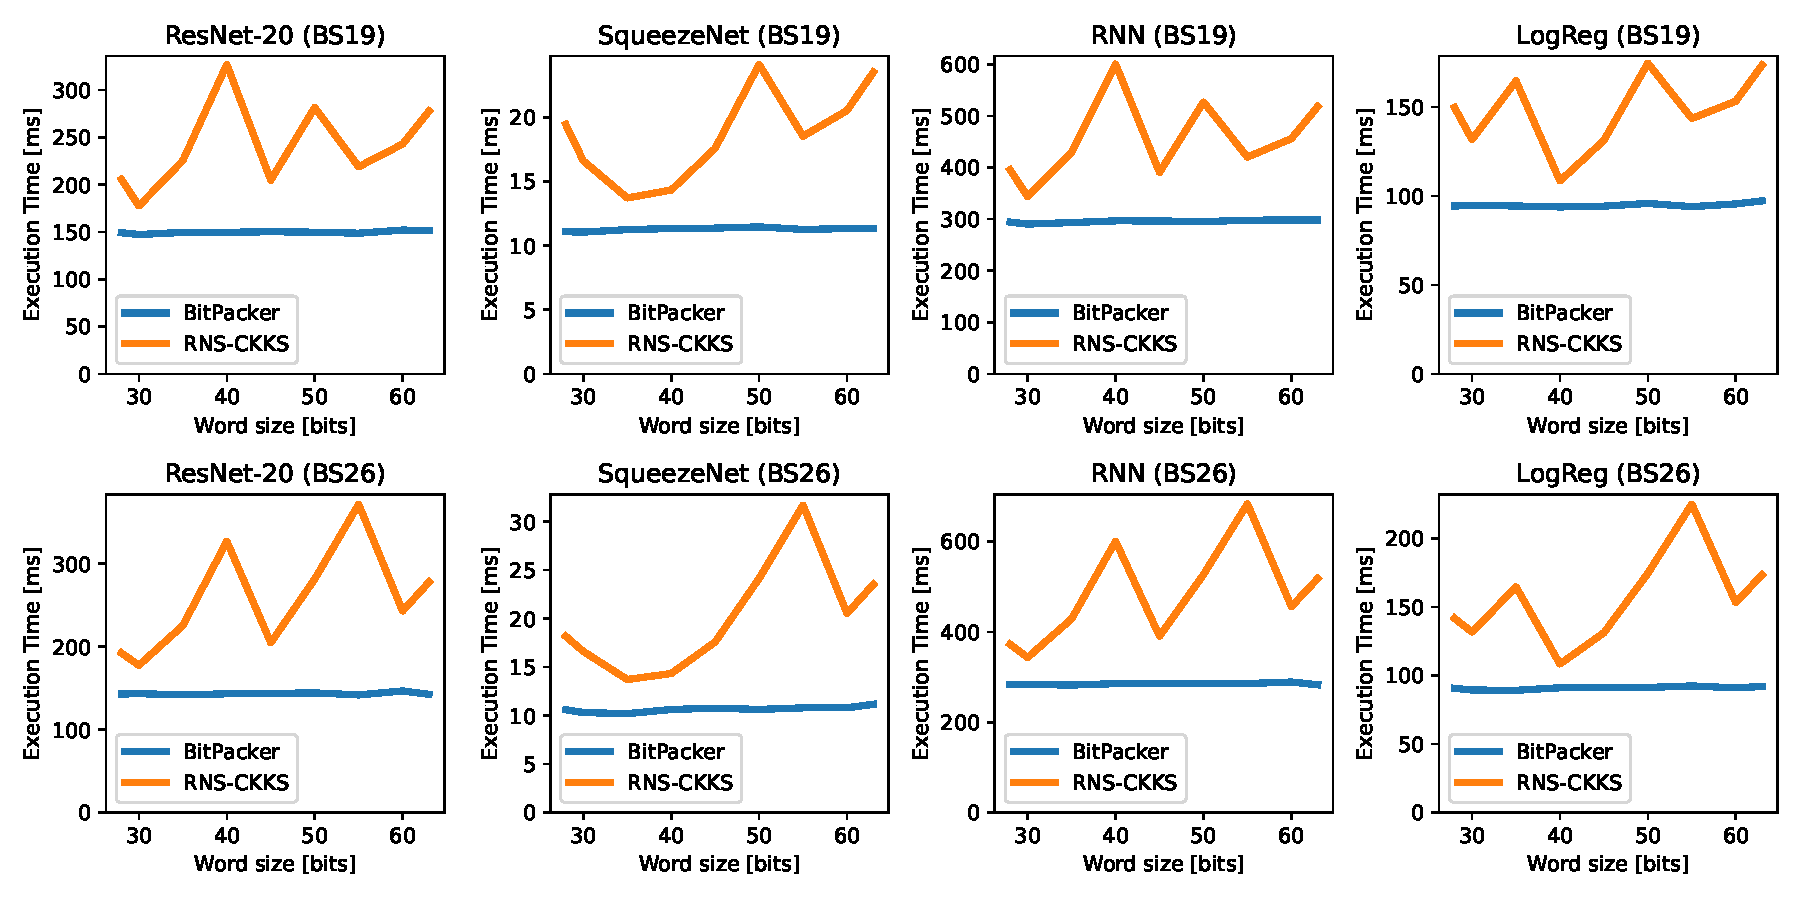
\includegraphics[width=\linewidth]{plots/performance.pdf}
            \caption{Execution time in milliseconds on CraterLake of \name
            compared to RNS-CKKS as word size changes.}
            \label{fig:bitwidthsweep}
        \end{center}
    \end{figure*}
}

\newcommand{\figAsymptotic}{
    \begin{figure}[t]
        \begin{center}
            \includegraphics[width=\columnwidth]{figures/ag_asymptotic.pdf}
            \caption{blah}
            \label{fig:asymptotic}
        \end{center}
    \end{figure}
}

\newcommand{\figNewLayout}{
    \begin{figure}[t]
        \begin{center}
            \includegraphics[width=\columnwidth]{figures/ag_new_layout.pdf}
            \caption{blah}
            \label{fig:newLayout}
        \end{center}
    \end{figure}
}

\newcommand{\figOldLayout}{
    \begin{figure}[t]
        \begin{center}
            \includegraphics[width=\columnwidth]{figures/ag_old_layout.pdf}
            \caption{blah}
            \label{fig:oldLayout}
        \end{center}
    \end{figure}
}

\newcommand{\figUsecase}{
    \begin{figure}[t]
        \begin{center}
            \includegraphics[width=\columnwidth]{figures/ag_usecase.pdf}
            \caption{blah}
            \label{fig:usecase}
        \end{center}
    \end{figure}
}

\newcommand{\figBreakdown}{
    \begin{figure}[t]
        \begin{center}
            \includegraphics[width=\columnwidth]{figures/ag_breakdown.pdf}
            \caption{blah}
            \label{fig:breakdown}
        \end{center}
    \end{figure}
}

\newcommand{\figRfSweep}{
    \begin{figure}[t]
        \begin{center}
            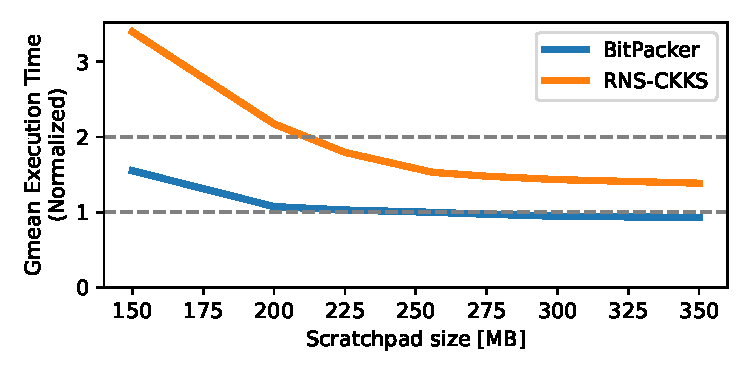
\includegraphics[width=\columnwidth]{plots/rf_sweep.pdf}
            \vspace{-0.3in}
            \caption{Gmean execution time on 28-bit CraterLake across register file sizes, relative to \name at 256\;MB.}
            \label{fig:rfSweep}
            \vspace{-0.2in}
        \end{center}
    \end{figure}
}

\newcommand{\figConstraints}{
\begin{figure}[t]
  \begin{center}
    \includegraphics[width=0.9\columnwidth]{figures/ag_constraints.pdf}
    \vspace{-0.08in}
    \caption{The modulus selection algorithm needs to take into account program and hardware constraints.
          Dashed arrows denote \emph{constrains}.}
    \label{fig:constraints}
    \vspace{-0.25in}
  \end{center}
\end{figure}
}

\newcommand{\figCraterLake}{
    \begin{figure}[b]
      \vspace{-0.1in}
      \begin{center}
        \includegraphics[width=0.7\columnwidth]{figures/ag_craterlake.pdf}
        \caption{Overview of CraterLake's architecture.}
        \label{fig:craterlake}
      \vspace{-0.15in}
      \end{center}
    \end{figure}
}

\newcommand{\figHomMult}{
    \begin{figure}[t]
      \begin{center}
        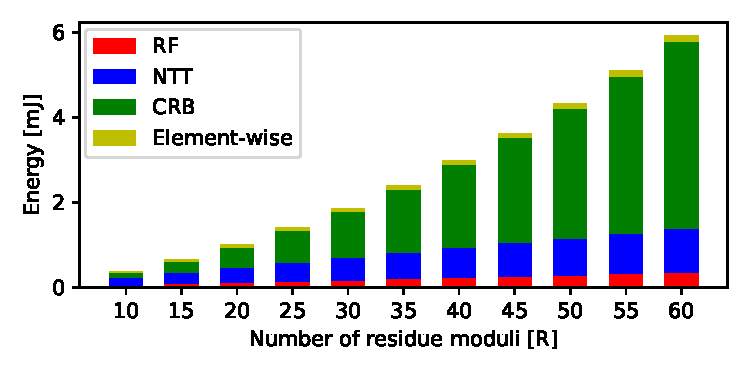
\includegraphics[width=0.95\columnwidth]{plots/hom_mult.pdf}
        \vspace{-0.2in}
        \caption{Energy breakdown for a homomorphic multiply as a function of residues $R$, for a 28-bit hardware word size.}
        \vspace{-0.25in}
        \label{fig:homMult}
      \end{center}
    \end{figure}
}

\newcommand{\figSawtooth}{
\begin{figure}[t]
  \begin{center}
    \includegraphics[width=0.9\columnwidth]{figures/ag_sawtooth.pdf}
    \vspace{-0.08in}
    \caption{Noise management affects ciphertext coefficient width ($\log_2Q$). Narrowing $\log_2Q$ after rescales trims noise;
    bootstrapping produces a low-noise, high-$\log_2Q$ ciphertext.}
    \label{fig:sawtooth}
    \vspace{-0.25in}
  \end{center}
\end{figure}
}

\newcommand{\figWordsizeSweep}{
    \begin{figure}[t]
        \begin{center}
            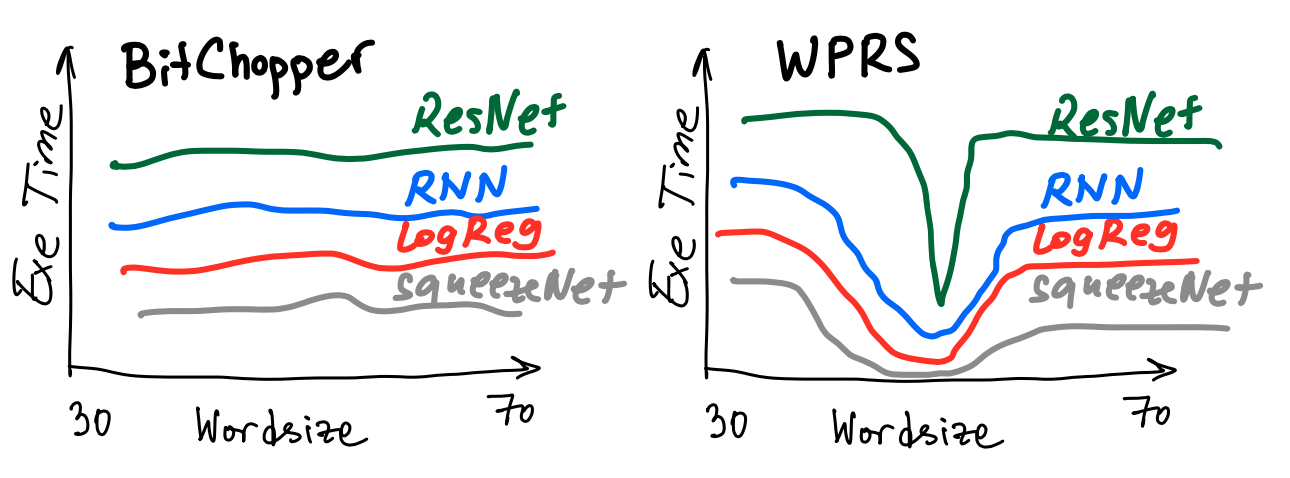
\includegraphics[width=\columnwidth]{plots/wordsize_sweep.png}
            \caption{blah.}
            \label{fig:wordsizesweep}
        \end{center}
    \end{figure}
}

\newcommand{\figIntro}{
\begin{figure}[t]
  \centering
    \includegraphics[width=0.99\columnwidth]{figures/ag_intro.pdf}
\vspace{-0.08in}
\caption{The state-of-the-art RNS-CKKS implementation leaves many bits of the
datapath unused, wasting area and energy, because it links residue size and 
scale (a). \name is a new RNS implementation
of CKKS that avoids this problem, achieving high utilization (b).}
\label{fig:intro}
\vspace{-0.15in}
\end{figure}
}

\newcommand{\figGmeanSlowdown}{
    \begin{figure}[t]
      \begin{center}
        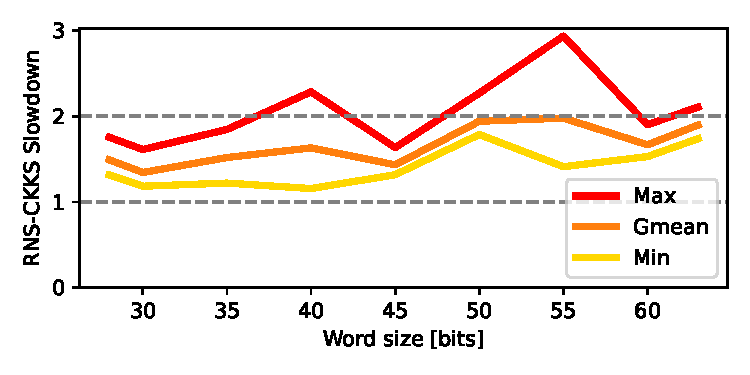
\includegraphics[width=\columnwidth]{plots/gmean_slowdown.pdf}
        \vspace{-0.3in}
        \caption{Gmean, maximum, and minimum slowdown for RNS-CKKS compared to \name across word sizes.}
        \label{fig:gmeanSlowdown}
        \vspace{-0.2in}
      \end{center}
    \end{figure}
}

\newcommand{\figGmeanPerformancePerArea}{
    \begin{figure}[t]
      \begin{center}
        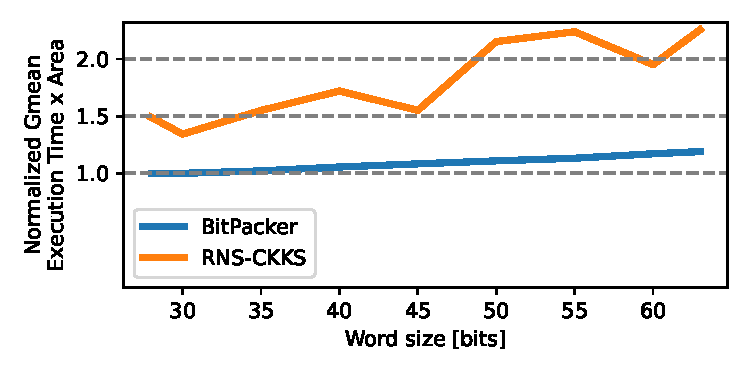
\includegraphics[width=\columnwidth]{plots/gmean_performance_per_area.pdf}
        \vspace{-0.3in}
        \caption{Gmean performance per unit area across word sizes for \name and RNS-CKKS.}
        \label{fig:gmeanPerformancePerArea}
        \vspace{-0.2in}
      \end{center}
    \end{figure}
}


\newcommand{\figResNetPerfAndErrVsLogScale}{
    \begin{figure}[t]
        \begin{center}
            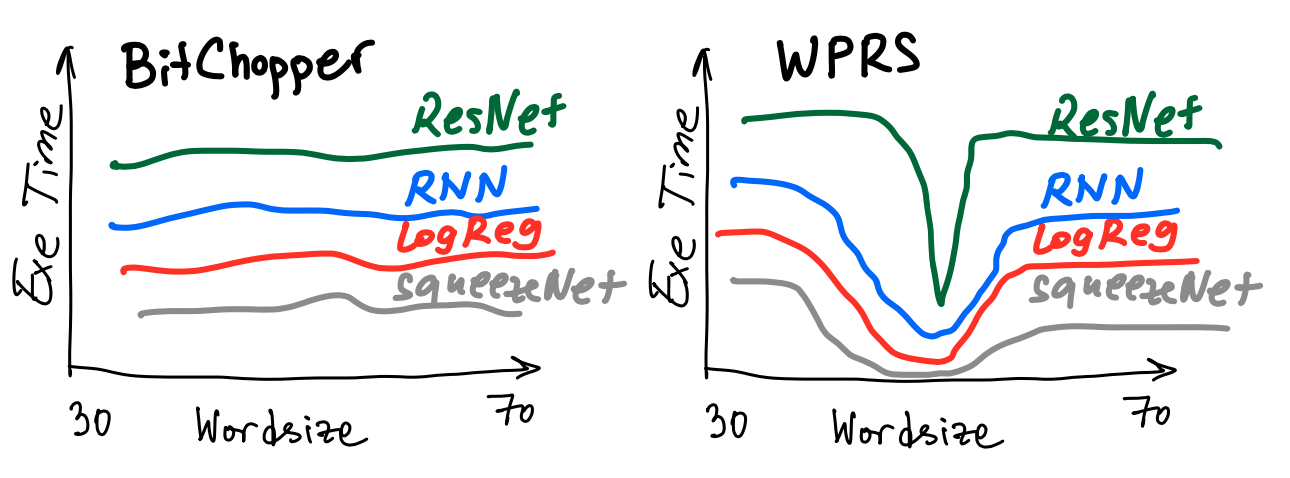
\includegraphics[width=\columnwidth]{plots/wordsize_sweep.png}
            \caption{blah.}
            \label{fig:resnetPerfAndErrVsLogScale}
        \end{center}
    \end{figure}
}

\newcommand{\figBpRescale}{
\begin{figure}[t]
    \begin{center}
        \includegraphics[width=\columnwidth]{figures/ag_rescale.pdf}
        \caption{Example showing how \name rescales the ciphertext from \autoref{fig:levels} from level $L=5$ to level $L-1=4$.}
        \label{fig:bpRescale}
    \end{center}
    \vspace{-0.25in}
\end{figure}
}

\newcommand{\figLevelsRnsCkks}{
\begin{figure}[t]
    \begin{center}
        \includegraphics[width=\columnwidth]{figures/ag_levels_rns_ckks.pdf}
        \vspace{-0.25in}
        \caption{Evolution of residue moduli and scales across three adjacent levels for RNS-CKKS.}
        \label{fig:levelsRnsCkks}
    \end{center}
    \vspace{-0.1in}
\end{figure}
}

\newcommand{\figLevelsBitPacker}{
\begin{figure}[t]
    \begin{center}
        % dsm:Sized width to match the size of the RNS-CKKS diagram.
        \includegraphics[width=0.89\columnwidth]{figures/ag_levels_bitpacker.pdf}
        \vspace{-0.1in}
        \caption{Evolution of moduli and scales across three adjacent levels for \name.}
        \label{fig:levels}
    \end{center}
    \vspace{-0.22in}
\end{figure}
}

\newcommand{\figBpModDown}{
\begin{figure}[t]
    \begin{center}
        \includegraphics[width=0.85\columnwidth]{figures/ag_mod_down.pdf}
        \caption{Example showing how \name mods-down the ciphertext from \autoref{fig:levels} from level $L=5$ to level $L-1=4$.}
        \vspace{-0.2in}
        \label{fig:bpModDown}
    \end{center}
\end{figure}
}

\newcommand{\tblNomenclature}{
    \newcolumntype{A}{>{\raggedright\arraybackslash}m{1.10in}}
    \newcolumntype{B}{>{\raggedright\arraybackslash}m{2.10in}}
    \begin{table}[t]
        \centering
        \begin{footnotesize}
        \begin{tabular}{@{}AB@{}}
        \toprule
        \textbf{} & \textbf{Description} \\
        \midrule
        \tpy{BigRns}
            & RNS representation of an integer \\
        \tpy{ResMod}
            & Residue modulus type \\
        \tpy{x.qs()}
            & all residue moduli of \tpy{BigRns} \tpy{x} \\
        \tpy{x.q()}
            & \mbox{the product of all residue moduli of}
            \tpy{RnsInt} \tpy{x} \\
        \tpy{prod(arr: Seq[int])}
            & product of integers in \tpy{arr} \\
        \tpy{x.drop(qi: ResMod)}
            & Drop \tpy{qi} and \tpy{x.r(qi)} from \tpy{x} \\
        \tpy{x.r(qi: ResMod)}
            & \mbox{Residue of \tpy{BigInt} \tpy{x}}
            corresponding to \tpy{ResMod} \tpy{qi} \\
        \tpy{inv(a, b)} & Inverse of \tpy{a} modulo \tpy{b} \\
        \tpy{ModMap}
            & The modulus map type \\
        \tpy{mm.S(lvl: int)}
            & \mbox{The scale at level \tpy{lvl} of}
            modulus map \tpy{mm} \\
        \tpy{Ct}
            & the ciphertext type \\
        \tpy{ct.0} / \tpy{ct.1} & \mbox{the first / second}
        polynomial of a \tpy{Ct} \\
        \tpy{Ct(ct0, ct1)} & Create a \tpy{Ct} \tpy{ct} with
        \tpy{ct.0 == ct0} and \tpy{ct.1 == ct1} \\
        \mbox{\tpy{x.add_r(y: int,}}
        \mbox{\tpy{  q: ResMod)}} & Add the residue modulus \tpy{q} and associates residue \tpy{y} to the \tpy{RnsInt} \tpy{x}. \\
        \bottomrule
        \end{tabular}
        \vspace{-0.05in}
        \caption{Pseudocode notation used in this paper.}
        \label{tbl:nomenclature}
        \vspace{-0.1in}
        \end{footnotesize}
    \end{table}
}

\newcommand{\tblScaleDivergence}{
    \begin{table}[t]
        \centering
        \footnotesize
        \begin{tabular}{r|rr|rr}
            \toprule
                  & \multicolumn{2}{c|}{Target} & \multicolumn{2}{c}{Actual} \\
            Level & $\log_2S$ & $\log_2 Q$ & $\log_2 Q$ & $\log_2S$ \\
            \midrule
            5     & 45              & 285             & 285.5           & 45.5 \\
            4     & 45              & 240             & 240.0           & 45.5 \\
            3     & 45              & 195             & 195.0           & 46.0 \\
            2     & 45              & 150             & 150.0           & 47.0 \\
            1     & 45              & 105             & 105.0           & 49.0 \\
            0     & 45              & 60              & 60.0            & 53.0 \\
            \bottomrule
        \end{tabular}
        \caption{An example run of the naive version of the greedy modulus chain generation algorithm that causes scale divergence. The mapping between levels and Target logscale are the inputs, and $Q_0=60$ are algorithm inputs.}
        \label{tbl:scaleDivergence}
    \end{table}
}

\newcommand{\figCkks}{
    \begin{figure}[t]
        \begin{center}
            \includegraphics[width=\columnwidth]{figures/ag_ckks.pdf}
            \vspace{-0.25in}
            \caption{Encryption process for CKKS.} % dsm: Not vector-based schemes in general...
            \label{fig:datatypes}
            \vspace{-0.25in}
        \end{center}
    \end{figure}
}

\newcommand{\tblComputeBreakdown}{
    \begin{table}[t]
        \centering
        \begin{tabular}{lrr}
            \toprule
                                        & \textbf{\% of keyswitching} & \textbf{\% of total} \\
            \midrule
            RNS Base Change             & 81.0\% & 70.0\%  \\
            NTTs                        & 19.0\% & 16.5\%      \\
            \midrule
            \textbf{Total Keyswitching} & & \textbf{86.5\%} \\
            \bottomrule
        \end{tabular}
        \caption{Percent of time spent on keyswitching during a homomorphic multiplication, as well as the breakdown of keyswitching between RNS Base Change and NTTs.}
    \end{table}
}
